\documentclass[letterpaper, 12pt]{article}

\usepackage{geometry}
 \geometry{
 letterpaper,
 total={170mm,257mm},
 left=20mm,
 top=20mm,
 bottom=20mm
 }
\usepackage{graphicx} % Required for inserting images
\usepackage{authblk}
\usepackage{amssymb}
\usepackage{lipsum}
\usepackage{float}
\usepackage{times}
\usepackage{amsmath}
\usepackage[format=plain,
            labelfont={bf,it},
            textfont=it]{caption}
\captionsetup{justification=raggedright,singlelinecheck=false}
\usepackage{ragged2e}
\usepackage{longtable}
\usepackage{comment}
\usepackage{setspace}
\usepackage{fancyhdr}
\usepackage{titlesec}
\usepackage[hyperindex,breaklinks]{hyperref}
\hypersetup{
    colorlinks=true,
    linkcolor=blue,
    filecolor=magenta,      
    urlcolor=blue,
    pdftitle={Overleaf Example},
    pdfpagemode=FullScreen,
    }
% \usepackage{background} % add COSIG logo to page
\usepackage[T1]{fontenc}
\usepackage{helvet}
\renewcommand{\familydefault}{\sfdefault}
\pagenumbering{gobble}
\usepackage[skip=10pt plus1pt, indent=40pt]{parskip}

\begin{comment}
\backgroundsetup{
   scale=1,
   angle=0,
   opacity=1,
   color=black,
   contents={\begin{tikzpicture}[remember picture, overlay]
      \node at ([xshift=3cm,yshift=1cm] current page.south west)
            {
\includegraphics[width = 5cm]{img/home/241017_final_logo_mockup.png}}; %<- change the name of image
     \end{tikzpicture}}
 }
\end{comment}

\titlespacing*{\section}
{0pt}{1.5ex plus 1ex minus .2ex}{1.3ex plus .2ex}

\renewcommand\Authfont{\fontsize{12}{14.4}\selectfont}
\renewcommand\Affilfont{\fontsize{9}{10.8}\itshape}

\begin{document}
\flushleft

\includegraphics[width=0.5\textwidth]{img/home/241017_final_logo_mockup.png}

\section*{Elemental composition}
\addcontentsline{toc}{section}{Elemental composition}
\textit{Last updated: 26 March 2025}

Different elements have different masses. For example, hydrogen has an atomic mass of 1.00784 u (atomic mass units), while oxygen has atomic mass of 15.999 u. Thus, although a molecule of water with molecular formula H$_2$O is composed of 66.6\% hydrogen and 33.3\% oxygen when counting atoms, it is 11.2\% hydrogen and 88.8\% oxygen by mass. These compositions are the water molecule's \textit{elemental atomic proportions} or \textit{atomic percentages} and the \textit{elemental mass proportions} or \textit{mass percentages} or \textit{weight percentages}, respectively.

Characterizing the elemental composition of a sample is an essential part of many chemistry and materials science studies. Elemental compositions are often determined by \href{https://en.wikipedia.org/wiki/Energy-dispersive_X-ray_spectroscopy}{energy dispersive x-ray spectroscopy (EDX/EDS/EDAX)} or \href{https://en.wikipedia.org/wiki/X-ray_photoelectron_spectroscopy}{X-ray photoelectron spectroscopy (XPS)}. You will often see these results provided in a table. In tables where both the atomic percentages and mass percentages for a compound/material are provided, they can be checked against one another. You can use \href{https://osf.io/gp4mf}{this spreadsheet} to convert between atomic percentages and mass percentages and vice-versa. These percentages can also be checked against what the authors claim the material is (see Example 3).

\subsection*{Isotopes}

Not all atoms of an element will have the same mass; different isotopes of an element can weigh different amounts. For example, the copper in the Earth's crust is about 69\% copper-63 (atomic mass 62.929 u) and about 31\% copper-65 (atomic mass 64.927 u). To account for the differing amounts of isotopes that will be found in a sample, chemists generally use a single \href{https://en.wikipedia.org/wiki/Standard_atomic_weight}{standard atomic weight} for each element. For copper, this value is 63.546 u (the weighted average of the atomic masses of the two copper isotopes commonly found in the Earth's crust).

Unless the authors of an article explicitly specify that they are quantifying the abundance of a specific isotope of an element, it is generally safe to use each element's standard atomic weight for fact-checking a composition table.

\subsection*{Should elemental composition percentages add up to 100\%?}

Techniques used for elemental composition quantification, like EDX, are associated with some analytical uncertainty. As a result, the elemental composition of a sample provided through EDX analysis may not add up to 100\%. The raw total of elemental composition percentages from EDX analysis is known as the ``analytical total'' (see the Discussion section of \href{https://doi.org/10.1007/s10853-024-10285-4}{Newbury and Ritchie, 2024}). 

Raw analytical totals can give an idea of the trustworthiness of an elemental analysis and should general fall between 98\% and 102\% (i.e., close to unity). Analytical totals far below 98\% can indicate that an element is present in a material but not included in the elemental composition analysis. 

Many authors, knowing that percentages \textit{should} add up to 100\%, will normalize their tables by this analytical total so that the reported percentages do add up to 100\%. This practice can conceal analytical errors and should generally be avoided.

In summary, elemental composition percentages that do not sum to 100\% but are otherwise close to 100\% are usually no cause for concern. However, elemental composition percentages that sum to a value far off from 100\% may be problematic.

\pagebreak

\subsection*{Example 1: No major issues with elemental composition table}

\href{https://doi.org/10.1080/10962247.2020.1813836}{Annamalai and Gurumurthy (2021)} report using EDX to quantify the elemental composition of electronic waste. In Table 4, the elemental weight percentages they report are entirely consistent with the elemental atomic percentages they report. There are no major issues with this analysis. However, the totals do add to up exactly 100\%, which suggests that this data has been normalized against the analytical total of elemental percentages. This practice can conceal analytical errors and is generally discouraged for EDX analysis.

\begin{figure}[h!tbp]
    \centering
    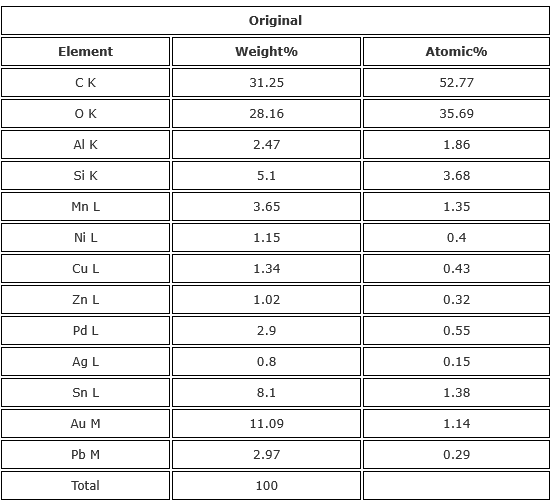
\includegraphics[width=0.8\textwidth]{img/elemental_composition/annamalai_gurumurthy_table_4.png}
    \caption*{An elemental composition table with no major detectable issues. Adapted from Table 4 of \href{https://doi.org/10.1080/10962247.2020.1813836}{Annamalai and Gurumurthy (2021)}.}
\end{figure}

\pagebreak

\subsection*{Example 2: Elemental atomic percentages do not match elemental weight/mass percentages}

\href{https://doi.org/10.1016/j.photonics.2020.100889}{Salim et al. (2021)} report using EDX to quantify the elemental composition of amorphous cinnamon nanoparticles. However, in the inset table of Figure 2C, the claimed elemental atomic percentages are incompatible with the claimed elemental weight/mass percentages.

\begin{table}[h!tbp]
\begin{center}
\begin{tabular}{c|c|c|c}
Element & Claimed Wt\% 	& Claimed At\% 	& Calculated At\%\\
\hline
Cu 	& 44.2 	& 38.4 	& 16.3\\
C 	& 27.7 	& 23.9 	& 54.2\\
O 	& 13.5 	& 13.5 	& 19.8\\
S 	& 8.1 	& 8.2 	& 5.9\\
Ca 	& 4.7 	& 5.6 	& 2.8\\
Fe 	& 1.3 	& 4.8 	& 0.5\\
Na 	& 0.3 	& 3.4 	& 0.3\\
K 	& 0.2 	& 2.2 	& 0.1\\
\end{tabular}
\end{center}
\end{table}

\begin{figure}[h!tbp]
    \centering
    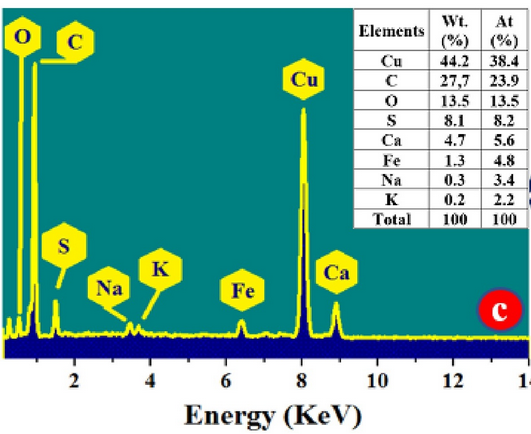
\includegraphics[width=0.8\textwidth]{img/elemental_composition/salim_table.png}
    \caption*{An elemental composition table where the claimed elemental atomic percentages are incompatible with the claimed elemental weight/mass percentages. Adapted from Figure 2C of \href{https://doi.org/10.1016/j.photonics.2020.100889}{Salim et al. (2021)}.}
\end{figure}

The EDX spectrum shown in this figure also has numerous issues. For more information, see the \href{https://osf.io/shfjy}{COSIG EDX guide}.

\subsection*{Example 3: Unexpected atomic percentages}

\href{https://doi.org/10.1371/journal.pone.0162891}{Mandizadeh et al. (2017)} report using EDX to confirm the elemental composition of SrCr$_x$Fe$_{12-x}$O$_{19}$ nanoceramics. However, for a sample that should have the molecular formula SrCr$_{0.5}$Fe$_{11.5}$O$_{19}$, they report the elemental atomic percentages as 3.95\% strontium, 64.27\% iron, 5.45\% chromium and 26.33\% oxygen. One would expect the oxygen proportion of their sample to be much closer to 19 oxygen atoms for every 32 atoms total ($\sim$ 59.4\%). The authors may have inadvertantly reported the elemental weight percentages as the elemental atomic percentages. Treating these percentages as the elemental weight percentages instead, we obtain a sample that is 1.5\% strontium, 39.1\% iron, 3.6\% chromium and 55.9\% oxygen by elemental atomic percentage, much closer to expectation.

\subsection*{Additional resources}

\begin{itemize}
    \setlength\itemsep{-0.5em}
    \item \href{https://doi.org/10.1007/s10853-024-10285-4}{``Testing the accuracy of low-beam-energy electron-excited X-ray microanalysis with energy-dispersive spectrometry'' (2024)}
    \item \href{https://doi.org/10.1017/S1431927619002964}{``Using the EDS Clues: Peak Fitting Residual Spectrum and Analytical Total'' (2019)}
    \item \href{https://doi.org/10.6028/jres.107.045}{``Limitations to Accuracy in Extracting Characteristic Line Intensities From X-Ray Spectra'' (2002)}
    \item \href{https://osf.io/shfjy}{COSIG: Energy-dispersive X-ray spectroscopy}
\end{itemize}

\end{document}